\chapter{
کاهش بعد و داده‌های بزرگ مقیاس
}


%========================================Section====================================
\section{
کاهش بعد
}
\subsection{
تحلیل مؤلفه‌های اصلی
}
\label{sec:ch2pca}

تحلیل چند متغیره معمولا بر روی داده‌هایی که شامل تعداد زیادی از متغیرهای مرتبط با هم هستند انجام می‌شود.
روش تحلیل مؤلفه‌های اصلی(
\lr{PCA}
)%
\LTRfootnote{principal components analysis}
 یک ابزار کاهش بعد است که می توان از آن برای کاهش یک مجموعه‌ی بزرگ از متغیرها به مجموعه‌ی کوچکتری که غالب اطلاعات مجموعه‌ی بزرگ را دارد استفاده کرد.

روش تحلیل مؤلفه‌های اصلی استفاده از یک تابع ریاضی است که تعدادی متغیر (احتمالا) همبسته را به تعداد (کمتر یا مساوی) متغیرهای غیرهمبسته به نام «مؤلفه‌های اصلی» تبدیل می‌کند.

بیشترین میزان اطلاعات ممکن در داده در اولین مؤلفه اصلی ثبت می‌شود. بیشترین میزان اطلاعات ممکن باقیمانده به ترتیب در مؤلفه‌های بعدی ثبت می‌شوند.

تحلیل مؤلفه‌های اصلی مشابه یک تابع چند متغیره دیگر به نام تحلیل عاملی است. این دو روش در موارد زیادی با یکدیگر اشتباه گرفته می‌شوند، و تفاوت بین این دو، و انواع تحلیل هایی که هر یک برایشان مناسب تر هستند به درستی تشخیص داده نمی‌شود.
به طور سنتی، تحلیل مؤلفه های اصلی بر روی ماتریس های متقارن مربعی انجام می شود. این ماتریس‌ها می تواند یکی از انواع
\lr{SSCP}%
\LTRfootnote{pure sums of squares and cross products}
 (مجموع خالص مربعات و ضرب های داخلی)، ماتریس کوواریانس%
\LTRfootnote{covariance}
 (مجموع مقیاس شده مربعات و ضرب های داخلی)، یا ماتریس همبستگی%
\LTRfootnote{correlation}
 (مجموع مربعات و ضرب های داخلی داده های استاندارد شده) باشد.

نتایج تحلیل روی ماتریس‌های از نوع
\lr{SSCP}
 و کوواریانس تغییری ندارند، چرا که تغییرات آنها فقط در یک ضریب مقیاس قابل مشاهده است.


\subsubsection{
اهداف تحلیل مؤلفه‌های اصلی   
}

تحلیل مؤلفه‌های اصلی فضای مشخصه‌ها را از تعداد زیادی متغیر به تعداد کمتری عامل کاهش می‌دهد، و یک تابع «غیر وابسته» است (یعنی نیازی وجود ندارد که یک متغیر وابسته تعیین شده باشد).
تحلیل مؤلفه های اصلی یک روش کاهش یا فشرده سازی ابعاد است. هدف، کاهش بعد است و تضمینی وجود ندارد که این ابعاد قابل تفسیر باشند.
در نهایت، انتظار آن است که زیرمجموعه‌ای از متغیرها از یک مجموعه بزرگتر انتخاب شود، به گونه‌ای که متغیرهای اولیه بیشترین همبستگی را با مؤلفه اصلی داشته باشند.

تحلیل مؤلفه‌های اصلی به دنبال رسیدن به ترکیبی خطی از متغیرها است، به گونه ای که بیشینه واریانس از آنها قابل استخراج باشد. پس از آن، این واریانس حذف شده و ترکیب خطی دومی جستجو می‌شود که بیشینه باقی‌مانده واریانس را توصیف می‌کند، و این روند ادامه پیدا می کند. به این روش، روش محور اصلی گفته می شود و عامل های متعامد غیرهمبسته را به دست می‌دهد. تحلیل مؤلفه‌های اصلی، واریانس (مشترک و یکتای) کل را شرح می‌دهند.

\textbf{
ویژه بردارها:
} مؤلفه‌های اصلی، هر دو واریانس مشترک و یکتای متغیرها را منعکس می‌کنند و بنابراین ممکن است که این روش به عنوان یک روش واریانس محور دیده شود که هم به دنبال بازتولید واریانس متغیر کل با تمام مؤلفه‌ها و هم بازتولید همبستگی‌ها است.
مؤلفه های اصلی، ترکیب های خطی از متغیرهای اولیه هستند که بر اساس میزان سهمشان در به وجود آمدن واریانس در یک بعد متعامد مشخص، وزن دهی می‌شوند. وزن‌های داده شده برای هر یک از مؤلفه‌های اصلی نسبت به داده‌های اولیه، ویژه بردارها هستند.

\textbf{
ویژه مقدارها:
}
 ویژه مقدار یک مؤلفه، واریانس همه‌ی متغیرهایی را که به آن عامل مرتبط هستند اندازه گیری می کند.
نسبت ویژه مقدارها، نسبت اهمیت توصیفی عامل ها با توجه به متغیرها است. اگر یک عامل دارای ویژه مقدار پایین باشد، نشانگر آن است که اثر کمی روی توصیف واریانس در متغیرها دارد، و ممکن است از آن در مقابل عامل های مهمتر چشم پوشی شود.
در ویژه مقدارها میزان تغییر در نمونه کل حساب شده است.

ویژه مقدار یک عامل ممکن است حاصل جمع مربعات عامل های تمامی متغیرها باشد. باید توجه شود که ویژه مقدارهای مرتبط با راه حل های دورانی و غیردورانی متفاوت خواهند بود، اگرچه مقدار کل آنها یکسان است.

برای به دست آوردن واریانس همه متغیرها که توسط عامل لحاظ می شود، مجموع مربعات بارگذاری های عامل برای آن عامل (ستون) را جمع کرده، و بر تعداد متغیرها تقسیم می کنیم. (توجه کنید که تعداد متغیرها برابر با مجموع واریانس آنهاست، چرا که واریانس یک متغیر استاندارد شده مساوی با ۱ است). این کار مشابه تقسیم ویژه مقدار عامل بر تعداد متغیرها است.

امتیاز 
\lr{PC}
: این امتیازها، امتیازهای هر نمونه (ردیف) در هر عامل (ستون) هستند. امتیاز عامل برای یک نمونه و برای یک عامل داده شده، به صورت مجموع حاصل ضرب  امتیاز استاندارد نمونه در هر متغیر با بارگذاری عامل مربوطه برای عامل داده شده محاسبه می‌شود.
\cite{site_pca}


%=======================================Section====================================
\section{
خوشه‌بندی و شاخص‌های سنجش
‌}
\subsection{
شاخص رند تعدیل شده
\label{sec:ARI}
}

برای مقایسه نتایج خوشه‌بندی در کنار شاخص‌های بیرونی، نیازمند معیارهای مورد توافق هستیم.
برای مجموعه‌ی 
$n$
 عضوی 
$S = \{O_1, \ldots, O_n\}$
، فرض کنید که
$U = \{u_1, \ldots, u_R\}$
 و
$V = \{v_1, \ldots, v_R\}$
 نمایانگر دو افراز متفاوت از عضوهای $S$  هستند ‌به گونه ای که 
$\bigcup_{i=1}^R u_i = S = \bigcup_{j=1}^C v_j$
 و 
$u_i \cap u_{i'} = \emptyset = v_j \cap v_{j'}$
برای 
$1 \leq i \neq i' \leq R$
و 
$1 \leq j \neq j' \leq C$
. فرض کنید که $U$ شاخص خارجی و $V$ نتیجه خوشه‌بندی است. فرض کنید $a$ تعداد جفت عضوهایی باشد که در یک کلاس یکسان $U$ و خوشه یکسان $V$ هستند، $b$ تعداد جفت عضوهایی باشد که در یک کلاس یکسان $U$ اما خوشه متفاوت $V$ هستند، $c$ تعداد جفت عضوهایی باشد که در یک کلاس متفاوت $U$ و خوشه یکسان $V$ هستند، و $d$ تعداد جفت عضوهایی باشد که در یک کلاس متفاوت $U$ و خوشه متفاوت $V$ هستند. می‌توان مقادیر $a$ و $d$ را به عنوان موارد توافق، و مقادیر $b$ و $c$ را به عنوان موارد عدم توافق تعریف کرد. شاخص رند%
\LTRfootnote{Rand index}
\cite{rand1971objective}
به سادگی به صورت 
$\frac{a+b}{a+b+c+d}$
 تعریف می‌شود. شاخص رند عددی بین ۰ و ۱ است. زمانی که دو خوشه کاملا در حالت توافق باشند، مقدار شاخص رند برابر با ۱ خواهد بود.

یکی از مشکلات شاخص رند آن است که مقدار مورد انتظار شاخص رند دو خوشه تصادفی یک مقدار ثابت (به عنوان مثال صفر) نیست. مقدار شاخص رند تعدیل شده%
\LTRfootnote{adjusted Rand index}
 پیشنهادی توسط هوبرت و اربی%
\LTRfootnote{Hubert and Arabie}
\cite{hubert1985comparing}
 بر پایه این فرض است که توزیع فوق‌هندسی%
\LTRfootnote{hypergeometric}
 تعمیم یافته برای مدل تصادفی استفاده می‌شود، به عبارت دیگر خوشه های $U$ و $V$ به شکلی تصادفی انتخاب می‌شوند که تعداد عضوهای کلاس‌ها و خوشه‌ها ثابت باشد. فرض کنید 
$n_{ij}$
 تعداد عضوهایی باشد که هم در کلاس 
$u_i$
 و هم در خوشه 
$v_j$
 هستند. در نظر بگیرید 
$n_{i.}$
 و 
$n_{.j}$ 
به ترتیب تعداد اعضا در کلاس
$u_i$
و خوشه‌ی
$v_i$
هستند. تمامی این نشانه‌گزاری‌ها در جدول
\autoref{tab:1iY}
بیان شده‌اند.

\begin{table}[h]
\caption{
نشانه‌گزاری برای جدول پیشایندی مقایسه دو بخش
}
\centering
\bigskip
\begin{latin}
\begin{tabular}{l|llll|l}
Class \textbackslash Cluster & $v_1$    & $v_2$  & $\ldots$ & $v_C$  & Sums      \\ \hline
$u_1$                        & $n_{11}$ & $n_{12}$ & $\ldots$ & $n_{1C}$ & $n_{1.}$     \\
$u_2$                        & $n_{21}$ & $n_{22}$ & $\ldots$ & $n_{2C}$ & $n_{2.}$     \\
$\vdots$                     & $\vdots$ & $\vdots$ & $\ddots$ & $\vdots$ & $\vdots$     \\
$u_R$                        & $n_{R1}$ & $n_{R2}$ & $\ldots$ & $n_{RC}$ & $n_{R.}$     \\ \hline
Sums                         & $n_{.1}$ & $n_{.2}$ & $\ldots$ & $n_{.C}$ & $n_{..} = n$
\end{tabular}
\end{latin}
\label{tab:1iY}
\end{table}

شکل کلی شاخص با در نظر گرفتن مقادیر انتظاری ثابت بدین شکل است که 
$\frac{\text{شاخص} - \text{مقدار مورد انتظار شاخص} }
{\text{حداکثر شاخص} - \text{مقدار مورد انتظار شاخص} }$
که از بالا به یک محدود است و زمانی که شاخص مقدار مورد انتظار را داشته باشد صفر می‌شود.

بر اساس مدل جنرال فوق‌هندسی، می‌توان نشان داد
\cite{ari1985}
:

\begin{align}
E \left[ \sum_{i,j} \binom{n_{ij}}{2} \right] 
= \left[ \sum_i \binom{n_{i.}}{2} \sum_j \binom{n_{.j}}{2} \right] / \binom{n}{2}
\label{eq:1iw}
\end{align}

عبارت 
$a+b$
می‌تواند به تبدیل خطی 
$\sum_{i,j} \binom{n_{ij}}{2}$
ساده‌سازی شود. شاخص رند تعدیل شده می‌تواند به شکل زیر ساده‌سازی شود:
\cite{ari1985}

\begin{align}
\frac{ 
	\sum_{i,j} \binom{n_{ij}}{2}
	-
	\left[ \sum_i \binom{n_{i.}}{2} \sum_j \binom{n_{.j}}{2} \right] / \binom{n}{2}
 }{
	\frac{1}{2} 
	\left[ 
		\sum_i 
		\binom{n_{i.}}{2}
		+
		\sum_j
		\binom{n_{.j}}{2}
	\right]
	-
	\left[ \sum_i \binom{n_{i.}}{2} \sum_j \binom{n_{.j}}{2} \right] / \binom{n}{2}
}
\label{eq:1ix}
\end{align}

با مثالی به بیان تعدیل انجام شده می‌پردازیم. 
\autoref{tab:1iy}
یک جدول پیشایندی به شکل جدول پیشایند در 
\autoref{tab:1iY}
است.

\begin{table}[h]
\caption{
مثال ۱ بررسی شاخص رند تعدیل شده در یک حالت ساده
}
\centering
\bigskip
\begin{latin}
\begin{tabular}{l|lll|l}
\textit{Class} \textbackslash \textit{Cluster} & $v_1$    & $v_2$  & $v_3$  & $\mathit{Sums}$  	\\ \hline
$u_1$                        & 1 	& 1	 & 0	  & 2 		\\
$u_2$                        & 1 	& 2	 & 1	  & 4		\\
$u_3$                        & 0	& 0	 & 4	  & 4		\\ \hline
$\mathit{Sums}$                         & 2	& 3	 & 5	  & $n$ = 10
\end{tabular}
\end{latin}
\label{tab:1iy}
\end{table}

$a$
به عنوان تعداد جفت اشیاء‌ی در که یک رده در 
$U$
و یک خوشه در 
$V$
قرار دارند. بنابراین 
$a$
می‌تواند به شکل 
$\sum_{i,j} \binom{n{ij}}{2}$
نوشته شود. در مثال 
\autoref{tab:1iy}
،
$a = \binom{2}{2} + \binom{4}{2} = 7$
. 
$b$
به عنوان تعداد جفت اشیاءی که هر دو در یک رده هستند در 
$U$
ولی در 
$V$
در دو خوشه‌ی متفاوت جای دارند. 
با توجه به الگوی نوشتار 
\autoref{tab:1iY}
$b$ 
را می‌تواند به شکل 
$\sum_i \binom{n_i}{2} - \sum_{i,j} \binom{n_{ij}}{2}$
بازنویسی کرد. در مثال 
\autoref{tab:1iy}
،
$b = \binom{2}{2} + \binom{4}{2} + \binom{4}{2} - 7 = 6$%
. همچنین
 $c$
به طور مشابه تعداد جفت اشیاءی که در یک خوشه در 
$V$
قرار دارند ولی در یک رده در 
$U$
قرار ندارند، تعریف می‌شود. پس 
$c$
به شکل 
$\sum_j \binom{n_{.j}}{2} - \sum_{i,j} \binom{n_{ij}}{2} = \binom{2}{2} + \binom{3}{2} + \binom{5}{2} - 7 = 7$%
. و 
$d$
تعداد جفت اشیاءی است که نه در 
‌$U$
در یک رده قرار دارند و نه در 
$V$
در یک خوشه. از آنجا که 
$a+b+c+d = \binom{n}{2}$
پس
$d = \binom{10}{2} -7 -6 -7 = 25$%
. شاخص رند برای مقایسه دو بخش در مثال 
\autoref{tab:1iy}
$ \frac{7+25}{45} = 0.711 $
است. در حالی که شاخص رند تعدیل شده،
$ \frac{7 - 14 \times 13 / 45}{(14+13)/2 - 14 \times 13 / 45} = 0.313$
(برای تعریف شاخص رند تعدیل شده به رابطه‌ی (%
\ref{eq:1ix}%
) مراجعه کنید). شاخص رند بسیار بیشتر از شاخص رند تعدیل شده است، که این موضوع معمولی است. از آنجا که شاخص رند بین $0$ و $1$ است، مقدار مورد انتظار شاخص رند (که مقداری ثابت نیست) باید بزرگتر مساوی ۰ باشد. از طرفی دیگر، مقدار مورد انتظار شاخص رند تعدیل شده $0$ است و بیشترین مقدار آن هم $1$ می‌باشد. بنابراین، محدوده‌ی بیشتری از مقادیر توسط  شاخص رند تعدیل شده بیان می‌شوند و حساسیت شاخص زیاد می‌شود.

در 
\cite{ari1986}%
، اندیس‌های مختلفی برای تطابق دو تفکیک مختلف در خوشه‌بندی و برای تعداد مختلفی خوشه مورد بررسی قرار گرفته‌اند و پیشنهاد آن‌ها شاخص رند تعدیل شده بود. ما شاخص رند تعدیل شده را به عنوان سنجه‌ای برای توافق معیار خارجی و نتایج خوشه‌بندی قرار دادیم.
\cite{yeung2001details}
\bigskip

%========================================Section===================================
\section{داده‌های حجیم}
عبارات زیر از سایت 
\lr{\textit{Information Week}}
نقل قول شده‌اند
\cite{site_iw}
:

\begin{itemize}
\item
مقدار داده‌ای که توسط کسب و کارها ذخیره می‌شود تقریبا هر ۱۲ تا ۱۸ ماه دو برابر می‌شود.
\item
پایگاه داده‌ها بیشتر هم ‌زمان شده‌اند. فروشگاه‌های زنجیره‌ای 
\lr{Wall-Marat}
داده‌های فروش را هر ساعت به روز می‌کند.
\item
اضافه شدن یک میلیون خط داده اجازه جستجوهای پیچیده‌تری را می‌دهد. شرکت 
\lr{eBay}
به کارمندان اجازه می‌دهد برای بدست آوردن درکی عمیق‌تر در خصوص رفتار مشتریان در میان داده‌های حراج در بازه‌های زمانی کوتاه جستجو کنند.
\item
بزرگترین پایگاه داده‌ها توسط، مرکز شتابدهنده خطی استاندارد، مرکز تحقیقات ناسا، آژانس امنیت ملی و ... در ابعادی در محدوده‌ی پتابایت (هزار ترابایت 
$10^{15}$
بایت)، اداره می‌شوند.
\end{itemize}

پدیده نو ظهور مجموعه‌ داده‌های حجیم، چالش‌های محاسباتی در بسیاری کاربردهای علمی و تجاری به وجود آورده است. شامل اخترفیزیک، بیوتکنولوزی، جمعیت شناسی%
\LTRfootnote{demographics}
، مالی، سیستم‌های اطلاعات جغرافیایی، دولت، دارو، ارتباطات از راه دور، محیط زیست، اینترنت.

\subsection{داده‌های حجیم وب}

وب چقدر بزرگ است؟  
\autoref{tab:searchengin}
نشان‌دهنده تعداد بازدید صفحات در موتورهای جستجوی امروزی است. به طور تخمینی حدود 
$D = 10^{10}$
صفحه‌ی وب را می‌توان بر اساس بازدید دو واژه‌ی بسیار پر کاربرد «
\lr{A}
» و «
\lr{THE}
» تخمین زد. 
\autoref{tab:searchengin}
 همچنین نشان می‌دهد که حتی کلماتی که به ندرت کاربرد دارند هم تعداد زیادی بازدید دارند.

\begin{table}[h]
\caption{
تعداد بازدید صفحات برای کلمات با بازخورد بالا و کلمات با بازخورد نادر
}
\centering
\bigskip
\begin{latin}
\begin{tabular}{lll}
\hline
Query        & Google         & Bing        \\ \hhline{===}
A            & 25,270,000,000 & 175,000,000 \\
The          & 25,270,000,000 & 101,000,000 \\
Kalevala     & 7,440,000      & 939,000     \\
Griseofulvin & 1,163,000      & 332,000     \\
Saccade      & 1,030,000      & 388,000     \\
\hline
\end{tabular}
\end{latin}
\label{tab:searchengin}
\end{table}


کلماتی با بازخورد معمولی چه میزان بازدید دارند؟ برای جواب این سوال ما به طور تصادفی ۱۵ صفحه از لغتنامه‌‌ی آموزشی انتخاب می‌کنیم.
\cite{litez94}
(لغتنامه‌ای با ۵۷،۱۰۰ کلمه) و اولین کلمه در هر صفحه را مد نظر قرار می‌دهیم. میانه‌ی آماری بر اساس جستجو‌گر گوگل ۱۰ میلیون صفحه برای کلمه است.

زبان انگلیسی چند کلمه دارد؟ در اینجا عبارتی را از 
\lr{AskOxford.com}
نقل قول می‌کنیم:

« این بیان می‌دارد که حداقل یک چهارم میلیون واژه‌ی انگلیسی مستقل وجود دارد. به جز افعال صرفی و کلمات فنی و ناحیه‌ای که توسط 
\lr{OED}%
\LTRfootnote{Oxford english dictionary}
تحت پوشش قرار نمی‌گیرند یا کلماتی که هنوز به لغتنامه‌های منتشر شده اضافه نشده‌اند. در صورتی که این موارد هم در نظر گرفته شوند تعداد لغات در حدود سه چهارم میلیون لغت خواهد بود »

بنابراین اگر یک ماتریس «عبارت به سند» 
$\mathbf{A} \in \mathbb{R}^{n \times D}$
در نظر بگیریم. در ابعاد وب این ماتریس در ابعاد 
$n \approx 10^6$
و 
$D \approx 10^{10}$
بزرگ خواهد شد.
در اینجا عدد 
$(i,j)$
در 
$\mathbf{A}$
تعداد ظهور واژه 
$i$
در سند 
$j$
را نشان می‌دهد.

کارکردن با ماتربسی در این ابعاد بزرگ چالش برانگیز است. برای مثال، شاخص 
\lr{LSI}%
\LTRfootnote{latent semantic indexing}
\cite{litez58}
و یک مدل موضوعی فراگیر، از 
\lr{SVD}%
\LTRfootnote{singular value decomposition}
بر روی ماتریس عبارت به سند استفاده می‌کند. که انجام این عملیات در ابعاد وب قطعا غیرممکن است.

یک مشکل اصلی در قبال مجموعه داده‌های سنگین، حافظه کامپیوتر است. به این دلیل که ابعاد و سرعت حافظه فیزیکی بسیار رشد کمتری در مقایسه با پردازنده‌ها (
\lr{CPU}
) دارد. این پدیده به عنوان دیوار حافظه شناخته می‌شود
\cite{litez139, litez168}
. برای مثال،‌ هر چند ممکن است تمامی رخداد‌های همزمان دوتایی از پیش محاسبه شوند، ولی نگهداری این حجم از داده در حافظه غیر ممکن است. علاوه بر این، گاهی اوقات تخصیص‌‌هایی با بیش از دو عامل هم اهمیت پیدا می‌کنند زیرا درخواست‌ها ممکن است شامل بیش از دو واژه هم باشند. یک راه حل ممکن این است که یک «نمونه» از 
$\mathbf{A}$
 نگهداری شود و همزمانی‌ها بر اساس این نمونه در حین کار تخمین زده شوند. ما حدس می‌زنیم که این روش توسط موتورهای جستجوی امروزی مورد استفاده قرار می‌گیرد، هر چند که روش واقعی قطعا جزو اسرار تجاری آن‌ها است.

هر چند که انتظار می‌رود تخمین‌ها سازگار باشند و فرکانس‌های جفت شده باید با افزایش عبارت به درخواست، کاهش پیدا کنند. 
\autoref{tab:querylengthcon}
نشان می‌دهد که تخمین‌های بیان شده با موتورهای جستجوی فعلی، همیشه سازگار نیستند.
\begin{table}[h]
\caption{
با افزایش تعداد عبارات در درخواست، باید فرکانس‌های جفت شده کاهش پیدا کنند. ولی تخمین‌های بیان شده توسط موتورهای جستجو گاهی این موضوع تثبیت شده را نقض می‌کنند.
}
\centering
\bigskip
\begin{latin}
\begin{tabular}{lll}
\hhline{===}
Query        				& Hits(Bing)    & Hits(Google) 	\\ \hline
America            			& 150,731,182 	& 393,000,000 	\\
America \& China          		& 15,240,116  	& 66,000,000 	\\
America \& China \& Britain     	& 235,111     	& 6,090,000     \\
America \& CHina \& Britain \& Japan 	& 154,444     	& 23,300,000    \\
\hhline{===}
\end{tabular}
\end{latin}
\label{tab:querylengthcon}
\end{table}

با اینکه، تعداد کل واژه‌های انگلیسی ( که به‌طور صحیح نوشته شده‌اند) هم اکنون شگفت‌انگیز است، در بسیاری کاربردهای متن کاوی، ما باید با ابعاد بسیار بزرگتری سر و کار داشته باشیم. در حالی که یک سند ممکن است بیانگر برداری از تک واژه‌ها باشد (به عبارت دیگر، مدل کیسه لغات%
\LTRfootnote{bag-of-words}%
). معمولا بهتر است سند به عنوان یک بردار از لغات به صورت 
\lr{l}
پیوسته %
\LTRfootnote{l-shingles}
\cite{litez34}
بیان شود. برای مثال، با استفاده از مدل ۳ پیوسته، جمله‌ی
\lr{"It is a nice day"}
به مجموعه‌ی زیر تجزیه می‌شود. 
\lr{\{"it is a", "is a nice", "a nice day"\}}
این مدل به طور جشمگیری ابعداد داده‌ها را افزایش می‌دهد. به خاطر اینکه، اگر مجموعه‌ی 
$10^6$
تک لغت انگلیسی موجود داشته باشد. مدل ۳ پیوسته تعداد ابعاد را از 
$10^6$
به 
$10^{18}$
افزایش می‌دهد.

\subsection{
جریان‌ داده‌‌های حجیم
}

در بسیاری کاربردهای جدید پردازش داده، جریان‌های داده‌ی حجیم نقش بنیادی دارند. جریان‌های داده‌ای که از روترهای اینترنت، سوئیچ‌های تلفن، رصد اتمسفر، شبکه‌های سنسور، شرایط ترافیکی بزرگراهی، داده‌های مالی و غیره 
\cite{litez5, litez141, litez49, litez19, litez96, litez69, litez91}
حاصل می‌شوند.

برخلاف پایگاه‌ داده‌های سنتی، معمول نیست که جریان‌های داده‌ی حجیم (که با سرعت زیادی منتقل می‌شوند) در جای نگهداری شوند. بنابراین پردازش معمولا به طور همزمان انجام می‌شوند. برای مثال، گاهی اوقات «رصد تصویری» داده‌ها با رصد تغییرات زمانی برخی آماره‌ها کفایت می‌کند. برای مثال آماره‌های نظیر: مجموع، تعداد آیتم‌های مجزا، برخی نرم‌های 
$l_\alpha$
. در برخی کاربردها (برای مثال، طبقه‌بندی صدا/محتوا و جدا سازی) نیاز است یک مدل یادگیری آماری برای رده‌بندی%
\LTRfootnote{classification}
یا خوشه‌بندی%
\LTRfootnote{clustering}
جریان داده‌های حجیم تدوین شود. ولی معمولا فقط می‌توانیم یک‌بار داده‌ها را مورد بررسی قرار دهیم.

یک خاصیت مهم جریان‌های داده‌ای این است که دینامیک هستند. به عنوان یک مدل محبوب، جریان 
$u$
شامل ورودی‌های 
$(i, u_i)$
است که 
$i = 1 \mathrm{to} D$
. برای مثال،
$D = 2^{64}$
زمانی که جریان بیان‌گر 
\lr{IP}
آدرس‌ها است.%
\footnote{
هرچند ما بیشتر اوقات تعداد دقیق ابعاد (%
\lr{D}%
) یک جریان داده را نمی‌دانیم ولی در بیشتر کاربردها کافی است حد بالایی محافظه‌کارانه‌ای را در نظر بگیریم. برای مثال 
$D = 2^{64}$
زمانی که جریان بیانگر 
\lr{IP}
های ورودی است. همچنین این یکی از دلایلی است که داده‌ها بسیار پراکنده هستند. به این نکته توجه داشته باشید که ابعاد بسیار بزرک تاثیری در محاسبه‌ی فاصله‌ها و نمونه‌گیری طی الگوریتم‌های معرفی شده در این پایان‌نامه ندارد.
}
ورودی‌ها ممکن است به هر ترتیبی باشند و ممکن است مرتبا به روز شوند. ذات دینامیک جریان داده‌های حجیم فرآیند نمونه‌گیری را بسیار چالش‌برانگیزتر از زمانی ‌می‌کند که با داده‌های ایستا سر و کار داریم.

%========================================Section===================================
\section{
چالش‌های نمونه‌گیری از داده‌های حجیم
}

در حالی که مسائل جذاب و چالش‌برانگیزی با ورود داده‌های حجیم شکل گرفته‌اند، این پایان‌نامه بر روی توسعه‌ی روش‌های کاهش‌بعد برای محاسبه فاصله در داده‌هایی با ابعاد بسیار بالا با استفاده از حافظه محدود تمرکز دارد.

در کاربردهای مدل‌سازی آماری و یادگیری ماشین، در اغلب موارد به جای داده‌های اصلی به فاصله، به خصوص فاصله‌ی جفتی نیاز داریم. برای مثال، محاسبه ماتریس گرام%
\LTRfootnote{Gram matrix}
$\mathbf{AA^T}$
در آمار و یادگیری ماشین معمول است. 
$\mathbf{AA^T}$
بیانگر همه‌ی ضرب‌های داخلی دوتایی در ماتریس داده‌ی 
‌$\mathbf{A}$
است.

دو داده‌ی 
$u_1, u_2 \in \mathbb{R}^D$
داده شده‌اند. ضرب داخلی آن‌ها ( که با 
$a$
نمایش داده می‌شود) و 
$l_\alpha$
(که با 
$d_{(\alpha)}$
نمایش داده می‌شود)%
\footnote{
ما فاصله $l_\alpha$ را به صورت 
$d_{(\alpha)} = \sum_{i=1}^{D} \mathopen| u_1 - u_2 \mathclose|^\alpha$
تعریف کرده‌ایم. به جای اینکه به شکل
$\mathopen( \sum_{i=1}^{D} \mathopen| u_1 - u_2 \mathclose|^\alpha \mathclose)^{1/\alpha}$
تعریف کنیم. زیرا شکل اول در کاربردهای عملی عمومیت بیشتری دارد. برای مثال، لم 
\lr{JL}
، در ادبیات معمولا به شکل توان دو $l_2$ بیان می‌شود. 
$\sum_{i=1}^{D} \mathopen| u_1 - u_2 \mathclose|^2$
به جای 
$\mathopen( \sum_{i=1}^{D} \mathopen| u_1 - u_2 \mathclose|^2 \mathclose)^{1/2}$
. در این پایان‌نامه، ما برای سادگی 
$\sum_{i=1}^{D} \mathopen| u_1 - u_2 \mathclose|^2$
را «فاصله $l_2$» بیان می‌کنیم به جای «مربع فاصله‌ی $l_2$».
}
 با عبارات زیر تعریف می‌شوند:

\begin{align}
a=u_1^T u_2 = \sum_{i=1}^{D} u_{1,i} u_{2,i} \\
d_{(\alpha)} = \sum_{i=1}^{D} \mathopen| u_1 - u_2 \mathclose|^\alpha 
\label{eq:1hP}
\end{align}

به این نکته توجه داشته باشید که هم ضرب داخلی و هم فاصله به شکل جمع
$D$
جمله تعریف می‌شوند. بنابراین، زمانی که داده‌ها به اندازه‌ای بزرگ مقیاس هستند که نمی‌توان به طور کارا آن‌ها را مدیریت کرد، انتخاب تصادفی ابعاد خیلی عادی به نظر می‌رسد تا بتوان با انتخاب تصادفی 
$k$
عضو از 
$D$
جمله تخمینی از مجموع به دست آوریم
(با ضریب مقیاس 
$\frac{D}{k}$
). در خصوص ماتریس داده‌ی 
$\mathbf{A} \in \mathbb{R}^{n \times D}$
\textit{
انتخاب تصادفی ابعاد
}%
\LTRfootnote{random coordinate sampling}
، $k$ ستون را از ماتریس داده به طور یکنواخت و تصادفی انتخاب می‌کند.

کاهش بعد از این جهت سودمند است که هم دورهای کاری 
\lr{CPU}
را کاهش ‌می‌دهد و هم در حافظه صرفه‌جویی می‌کند. در کابردهای جدید، در اغلب موارد صرفه‌جویی در حافظه از اهمیت بیشتری برخوردار است. در نیم قرن گذشته گلوگاه‌ محاسباتی حافظه بوده است، نه پردازشگر. سرعت پردازشگرها با نرخ تقریبی ۷۵ درصد در سال رو به افزایش است. در حالی که سرعت حافظه تقریبا سالی ۷ درصد افزایش می‌یابد
\cite{litez139}
. این پدیده به عنوان «دیوار حافظه»%
\LTRfootnote{memory wall}
شناخته می‌شود.
‌\cite{litez139, litez168}
بنابراین در کاربردهایی که شامل مجموعه داده‌های حجیم می‌شوند، بحرانی‌ترین کار بیان کردن داده‌ها است. برای مثال،
از طریق کاهش بعد با فرمی فشرده برای قرارگیری در ابعاد حافظه در دسترس.


\subsection{
مزایای کاهش بعد با انتخاب تصادفی ابعاد
}

نمونه‌گیری تصادفی ابعاد به دو دلیلی معمولا انتخاب پیش‌فرض است.

\begin{itemize}
\item
\textbf{سادگی}
این روش از لحاظ زمانی تنها از مرتبه 
$O(nk)$
برای نمونه‌گیری 
$k$ 
ستون از 
$\mathbf{A} \in \mathbb{R}^{n \times D}$
طول می‌کشد.
\item
\textbf{انعطاف پذیری}
یک مجموعه نمونه را می‌توان برای تخمین بسیاری از شاخص‌های آماری استفاده کرد. شامل: ضرب داخلی، فاصله
$l_\alpha$
(برای هر مقداری از 
$\alpha$
)
\end{itemize}

\subsection{
معایب نمونه‌گیری تصادفی ابعاد
}
با این حال نمونه‌گیری تصادفی ابعاد دو ایراد اساسی دارد:
\begin{itemize}
\item
معمولا دقیق نیست زیرا مقادیری با مقدار زیاد محتمل است که گم شوند. مخصوصا زمانی که داده‌ها دم سنگینی داشته باشند. داده‌های بزرگ مقیاس دنیای واقعی (مخصوصا داده‌های مربوط به اینترنت) همیشه دم‌سنگین هستند و از قاعده توانی پیروی می‌کنند.
\cite{litez142,litez66, litez53, litez111}
زمانی که فاصله 
$l_2$
یا ضرب داخلی را تخمین می‌زنیم. واریانس تخمین‌ها بر اساس ممان چهارم داده‌ها تعیین می‌شود. در حالی که در داده‌های دم سنگین، گاهی اوقات حتی ممان اول هم معنی‌دار نیست (محدود نیست)
\cite{litez142}
.
\item
این روش داده‌های پراکنده را به خوبی مدیریت نمی‌کند. بسیاری از داده‌های بزرگ مقیاس به شدت پراکنده هستند، به عنوان مثال، داده‌های متنی 
\cite{litez60}
و داده‌های بر اساس بازار
\cite{litez7, litez158}
. به جز برخی واژه‌های کاربردی مانند 
\lr{"A"}
 و 
\lr{"The"}
بیشتر لغات با نسبت بسیار کمی در مستندات ظاهر می‌شوند (
$<1\%$
)
اگر ما داده‌ها را با در نظر گرفتن تعدادی از ستون‌های ثابت، کاهش بعد دهیم. خیلی محتمل است که بیشتر داده‌های (مقادیر غیر صفر) را از دست بدهیم.به خصوص موارد جذابی که در دو نمونه، دو ستون با هم غیر صفر شده‌اند.
\end{itemize}
در این پایان‌نامه ما روش نگاشت تصادفی را مورد بررسی قرار می‌دهیم و نشان خواهیم داد که این روش به خوبی قابلیت مدیریت داده‌های دم‌سنگین را دارد.

%========================================Section====================================
\section{نگاشت تصادفی پایدار}
\label{sec:srp}

\autoref{fig:matrixmulti}
، ایده نگاشت تصادفی را نشان می‌دهد. ایده اصلی نگاشت تصادفی ضرب ماتریس داده‌ی 
$\mathbf{A} \in \mathbb{R}^{n \times D}$
در ماتریس تصادفی 
$\mathbf{R} \in \mathbb{R}^{D \times k} (k \ll D)$
است. که حاصل ماتریس نگاشت شده‌ی 
$\mathbf{B} = \mathbf{A} \times \mathbf{R} \in \mathbb{R}^{n \times k}$
است. 
$\mathbf{B}$
بسیار کوچکتر از 
$\mathbf{A}$
است و بنابراین به راحتی قابل ذخیره‌سازی است. (برای مثال: برای حافظه‌های فیزیکی به اندازه‌ی کافی کوچک است)

\begin{figure}[h]
\centering
\begin{latin}
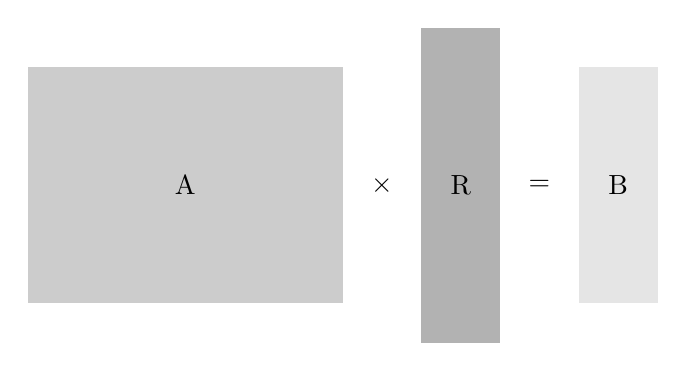
\begin{tikzpicture}
\fill[black!20!white] (0,1) rectangle (4,4);
\node at (2,2.5) [rectangle,preaction={fill=black!20},font={A}] {};
\node at (4.5,2.5) [rectangle,preaction={fill=black!0},font={$\times$}] {};
\fill[black!30!white] (5,0.5) rectangle (6,4.5);
\node at (5.5,2.5) [rectangle,preaction={fill=black!30},font={R}] {};
\node at (6.5,2.5) [rectangle,preaction={fill=black!0},font={=}] {};
\fill[black!10!white] (7,1) rectangle (8,4);
\node at (7.5,2.5) [rectangle,preaction={fill=black!10},font={B}] {};
\end{tikzpicture}
\end{latin}
\caption{
نگاشت تصادفی پایدار 
$\mathbf{B} = \mathbf{A} \times \mathbf{R}$
،
$\mathbf{A}$
ماتریس اولیه داده‌ها است.
}
\label{fig:matrixmulti}
\end{figure}

ماتریس نگاشت‌گر 
$\mathbf{R} \in \mathbb{R}^{D \times k}$
معمولا از داریه‌های مستقل هم توزیع (
\lr{i.i.d}
) یک توزیع متقارن $\alpha$-پایدار پر شده است.
\cite{litez171}
(بنابراین نام این روش «نگاشت تصادفی پایدار» است.)
بر اساس مشخصات توزیع‌های $\alpha$-پایدار، داده‌های نگاشت شده هم از توزیع $\alpha$-پایدار پیروی می‌کنند. که بر اساس آن‌ها شاخص‌های $l_\alpha$ و فاصله دودویی $l_\alpha$ در $\mathbf{A}$ تخمین زده می‌شوند و می‌توانیم داده‌های اصلی را دور بریزیم.

موفقیت نگاشت تصادفی پایدار توسط لم 
\lr{JL}%
\LTRfootnote{Johnson-Lindenstrauss}%
\cite{litez103}
برای کاهش بعد در $l_2$ نشان داده شده است. لم
\lr{JL}
بیان می‌کند: رعایت
$k = O \left ( \frac{\log n}{\epsilon^2 } \right ) $
تضمین می‌کند هر فاصله $l_2$ میان $n$ نقطه در هر تعداد بعدی با دقت 
$1\pm\epsilon$
 با احتمال بالایی تخمین زده شود. ($k$ در اینجا بیانگر تعداد ابعاد کاهش یافته است)

با این حال لم 
\lr{JL}
برای نرم‌های فاصله با 
$\alpha$
کوچکتر از ۲ 
$l_\alpha ( \alpha < 2 )$
صادق نیست. در صورتی که لازم باشد از برآوردگرهایی استفاده کنیم که متریک باشند (در نامساوی مثلثی صدق کنند). به این نتیجه «عدم امکان»%
\LTRfootnote{impossibility}
 گفته می‌شود.
\cite{litez39, litez109, litez33}
خوشبختانه شامل برآوردگرهایی که متریک نیستند نمی‌شود. در این پایان‌نامه ما در مورد برآوردگرهای گوناگونی که متریک نیستند صحبت خواهیم کرد. شامل: میانگین هندسی%
\LTRfootnote{geometric mean}
، میانگین هارمونیک%
‌\LTRfootnote{harmonic mean}
، توان نسبی%
\LTRfootnote{fractional power}
و همچنین حداکثر بزرگنمایی.

%=====================================Section===================================
\section{کاربردها}

علاقه‌ی زیادی به فنون کاهش بعد وجود دارد که در کاربردهای زیادی مورد استفاده قرار می‌گیرند. مانند: قانون وابستگی%
\LTRfootnote{association rules}
\cite{litez30, litez31}
، خوشه‌بندی، بهینه‌سازی درخواست%
\LTRfootnote{query optimization}
\cite{litez136, litez44}
، تشخیص تکراری%
\LTRfootnote{duplicate detection}
\cite{litez34, litez28}
و بسیاری موارد دیگر. روش‌های کاهش بعد هر چه بیشتر و بیشتر برای مجموعه‌های بزرگتر اهمیت پیدا می‌کنند.

طرح برودر%
\LTRfootnote{Broder's sketch}
\cite{litez34}
در ابتدا برای تشخیص صفحات وب تکراری معرفی شد. 
\lr{URL}%
های زیادی به 
\lr{HTML}%
های مشابه (یا تقریبا مشابه) اشاره می‌کنند. جواب‌های برآورد شده به اندازه‌ی کافی خوب بودند. نیازی نبود تا همه تکراری‌ها پیدا شوند ولی کاربردی بود که تعداد زیادی از آن‌ها پیدا شوند، بدون اینکه بیش از ارزش آن از توان محاسباتی استفاده شود.

در کاربردهای بازیابی اطلاعات (%
\lr{IR}%
)%
\LTRfootnote{information retrieval}
معمولا گلوگاه حافظه‌ی فیزیکی است. زیرا مجموعه‌ی وب برای حافظه (%
\lr{RAM}%
) بسیار بزرگ است و از طرفی ما می‌خواهیم زمان گشتن به دنبال داده‌ها بر روی دیسک را کمینه کنیم. زیرا زمان پاسخ به یک درخواست کلیدی است.
\cite{litez29}
 به عنوان یک وسیله صرفه‌جویی در فضا، کاهش بعد یک ارائه فشرده از داده‌ها فراهم می‌کند که برای تولید جواب‌های تخمینی در حافظه فیزیکی مورد استفاده قرار می‌گیرند.

ما به بازدید صفحات وب اشاره‌ کردیم. اگر ما یک عبارت جستجوی دو کلمه‌ای داشته باشیم، می‌خواهیم بدانیم چه تعداد از صفحات هر دو کلمه را دارند. فرض می‌کنیم محاسبه‌ی از قبل و نگهداری بازدید صفحات غیر ممکن باشد. حداقل نه برای کلماتی که تکرار زیادی ندارند و سری‌های چند کلمه‌ای.

مرسوم است که در بازیابی اطلاعات با یک ماتریس بزرگ عبارت به ازای سند شروع کنیم که در آن مقادیر ورودی نشان‌دهنده‌ی وجود عبارت در متن است. بنا به کاربردهای خاص می‌توانیم یک اندیس معکوس %
\LTRfootnote{inverted index}
بسازیم و کلیتی از عبارات (برای تخمین ارتباط لغات) یا اسناد (برای تخمین شباهت اسناد) نگهداری کنیم.

\subsection{
کاوش قوانین وابستگی
}
تحلیل‌های مبتنی بر بازار و قوانین وابستگی 
\cite{litez8, litez9, litez10}
ابزارهای مناسبی برای کاوش پایگاه‌ داده‌های تجاری هستند. پایگاه داده‌های تجاری روز به روز بزرگتر و تُنُک‌تر می‌شوند
\cite{litez7, litez158}
و الگوریتم‌های مختلف نمونه‌برداری برای آن‌ها، پیشنهاد شده است. نمونه برداری این امکان را فراهم می‌کند تا قواعد تخصیص را به صورت آنلاین برآورد کنیم، که می‌تواند مزایایی را در برخی کاربردهای خاص داشته باشد.

\subsection{
همه‌ی جفت تخصیص‌ها (فاصله‌ها)
}
در بسیاری از موارد کاربرد، شامل رده‌بندی فاصله محور یا خوشه‌بندی و مدل‌سازی زبان با بای‌گرام%
\LTRfootnote{bi-gram}
\cite{litez48}
ما نیازمند محاسبه‌ی همه‌ی جفت تخصیص‌ها (یا فاصله‌ها) هستیم. ماتریس داده‌ی 
$\mathbf{A}$
شامل 
$n$
سطر و 
$D$
ستون داده شده است. محاسبه‌ی مستقیم
$\mathbf{AA}^T$
، هزینه‌ای از مرتبه‌ی 
$O(n^2 D)$
دارد.در شرایطی که 
$\bar{f}$
را 
برابر با میانگین تعداد مقادیر غیر صفر در تمام سطرهای 
‌$\mathbf{A}$
در نظر بگیریم، 
این هزینه از مرتبه‌ی 
$O(n^2 \bar{f})$
است. محاسبه مستقیم می‌تواند بسیار زمان‌بر باشد. به علاوه، زمانی که ماتریس داده آنقدر بزرگ است که در حافظه فیزیکی جا نمی‌شود، محاسبه بیش از پیش ناکارآمد خواهد بود.


\subsection{
برآورد فاصله‌ها به طور آنلاین
}

در حالی که ماتریس داده‌ی اولیه 
$\mathbf{A} \in \mathbb{R}^{n \times D}$
ممکن است برای حافظه‌ی فیزیکی بسیار بزرگ باشد، نگهداری%
\LTRfootnote{materializing}
همه جفت فاصله‌ها و جفت تخصیص‌ها در 
$\mathbf{A}$
، فضای 
$O(n^2)$
را اشغال می‌کند. این می‌تواند برای حافظه‌ی فیزیکی بسیار بزرگ باشد. این در شرایطی است که وابستگی‌های چندتایی را کنار بگذاریم، که در نظر گرفتن ‌آن‌ها شرایط را بسیار سخت‌تر خواهد کرد. در بسیاری از کاربردها نظیر یادگیری برخط، سیستم‌های توصیه آنلاین، تحلیل‌های بازار برخط و موتورهای جستجو، بهتر است که برداشت‌ها%
\LTRfootnote{sketches}
در حافظه نگهداری شوند و همه‌ی فاصله‌ها به طور آنلاین، در زمانی که مورد نیاز باشد، محاسبه شوند.

\subsection{
بهینه‌سازی درخواست از پایگاه داده
}

در پایگاه داده‌ها یک وظیفه‌ی بسیار مهم تخمین تلاقی‌های% 
\LTRfootnote{joins}
چندراهی است، که تاثیر زیادی بر روی کارایی سیستم دارد.
\cite{litez81}
بر اساس تخمین دوراهی، سه‌راهی و حتی جوین‌هایی از مرتبه‌ی بالاتر، بهینه‌گرهای درخواست یک نقشه برای کمینه کردن تابع هزینه می‌سازند (برای مثال، نوشتن‌های میانی%
\LTRfootnote{intermediate writes}
). بهینه بودن اهمیت بسیاری دارد زیرا مثلا نمی‌خواهیم زمان بیشتری برای بهینه‌سازی نقشه نسبت به زمان اجرای آن تلف کنیم.

ما از مثال «%
\lr{Governator}%
» برای نمایش کاربرد تخمین دو و چند راهه برای بهینه کردن درخواست استفاده می‌کنیم.

\begin{table}[h]
\caption{
بازدید صفحات گزارش شده توسط گوگل
برای چهار کلمه و وابستگی‌های دو، سه و چهارتایی آن‌ها
}
\centering
\bigskip
\begin{latin}
\begin{tabular}{lll}
\hhline{===}
        		 & Query		& Hits(Google) 	\\ \hline
\multirow{4}{*}{One-way} & Austria  	& 88,200,000 	\\
			 & Governor  	& 37,300,000 	\\
			 & Schwarzenegger & 4,030,000 	\\
			 & Terminator	 & 3,480,000 	\\ \hline
\multirow{6}{*}{Two-way} & Governor \& Schwarzenegger  	& 1,220,000 	\\ 
			 & Governor \& Austria  	& 708,000 	\\
			 & Schwarzenegger \& Terminator & 504,000 	\\
			 & Terminator \& Austria  	& 171,000 	\\
			 & Governor \& Terminator  	& 132,000 	\\
			 & Schwarzenegger \& Austria  	& 120,000 	\\ \hline
\multirow{4}{*}{Tree-way} & Governor \& Schwarzenegger \& Terminator  	& 75,100 \\
			  & Governor \& Schwarzenegger \& Austria  	& 46,100 \\
			  & Schwarzenegger \& Terminator \& Austria 	& 16,000 \\
			  & Governor \& Terminator \& Austria 		& 11,500 \\ \hline
\multirow{1}{*}{Four-way} & Governor \& Schwarzenegger \& Terminator \& Austria & 6,930	\\
\hhline{===}
\end{tabular}
\end{latin}
\label{tab:governator}
\end{table}

\autoref{tab:governator}
بازدید صفحات را برای چهار کلمه و ترکیبات دو، سه، چهارتایی آن‌ها نشان می‌دهد. فرض کنیم بهینه‌ساز قصد استخراج نقشه برای درخواست:
$"\mathrm{Governor, Schwarzenegger, Terminator, Austria}"$
را داشته باشد. راه حل استاندارد این است که با عبارات با کمترین فراوانی شروع کند:
$(("\mathrm{Schwarzenegger}" \cap "\mathrm{Terminator}") \cap "\mathrm{Governor}") \cap "\mathrm{Austria}"$
این نقشه 
$579,100$
نوشتن میانی بعد از اولین و دومین جوین دارد. یک بهینه‌سازی می‌تواند 
$(("\mathrm{Schwarzenegger}" \cap "\mathrm{Austria}") \cap "\mathrm{Terminator}") \cap "\mathrm{Governor}"$
باشد که 
$579,100$
را به 
$136,000$
کاهش می‌دهد.


\subsection{
جستجوی نزدیکترین همسایه از مرتبه‌ی زیر خطی
}

محاسبه‌ی نزدیکترین همسایه در بسیاری کاربردها از اهمیت زیادی برخوردار است. با این حال، به دلیل «نفرین ابعاد»%
\LTRfootnote{curse of dimensionality}
راه حل فعلی برای پیدا کردن بهینه‌ی نزدیکترین همسایه‌ها (حتی به طور تقریبی) اصلا رضایت بخش نیست.
\cite{litez88, litez100}

به دلیل ملاحظات محاسباتی، دو شکل اصلی در جستجوی نزدیکترین همسایه‌ها وجود دارد. اول اینکه ماتریس اصلی داده‌ها 
$\mathbf{A} \in \mathbb{R}^{n \times D}$
ممکن است برای حافظه فیزیکی بسیار بزرگ باشد ولی اسکن کردن دیسک‌های سخت برای پیدا کردن نزدیکترین همسایه‌ها می‌تواند خیلی کند باشد. دوما، پیدا کردن نزدیکترین همسایه‌های یک داده ممکن است
$O(nD)$
هزینه‌بر باشد که می‌تواند به شدت زمان‌بر شود.

با این حال، روش کاهش ابعادی در این پایان‌نامه می‌تواند در حافظه صرفه‌جویی کند و سرعت محاسبات را افزایش دهد. برای مثال: وقتی ماتریس داده‌ی اولیه 
$\mathbf{A}$
به ماتریس داده‌ی 
$\mathbf{B} \in \mathbb{R}^{n \times k}$
کاهش می‌یابد. با این حال، 
$O(nk)$
 است و معمولا این درخواست وجود دارد که هزینه‌ی محاسباتی از 
$O(n)$
به 
$O(n^\gamma)$
برای 
$\gamma < 1$
کاهش پیدا کند، حداقل برای کاربردهای خاص.

دو گروه اصلی الگوریتم‌های زیر خطی برای محاسبه عبارتند از 
\lr{KD-Trees}
(و انواع آن)
\cite{litez79, litez80}
و 
\lr{LSH}%
\LTRfootnote{locality-sensitive hashing}
\cite{litez15, litez56, litez100}
این الگوریتم‌ها معمولا با یک فضای متریک کار می‌کنند (که در ان نامساوی مثلثی برقرار است). برای مثال، فضای 
$l_\alpha$
زمانی که 
$\alpha \geq 1$
باشد یک متریک است. زمانی که به دنبال نزدیکترین‌ همسایه‌ها در 
$l_\alpha$
(%
$\alpha > 1$%
) می‌گردیم، می‌توانیم (نسبتا به سادگی) فضای جستجو را به طور کاملا اساسی با استفاده از نامساوی مثلثی کاهش دهیم. به عبارت دیگر، نیازی نیست که همه 
$n$
نقطه داده‌ها را مورد بررسی قرار دهیم.

در داده‌هایی با ابعاد بسیار بزرگ، الگوریتم‌های زیر خطی موجود شامل 
\lr{KD-trees}
و 
\lr{LSH}
، عملکرد رضایت بخشی ندارند.  وقتی حافظه‌ی فیزیکی (به جای 
\lr{CPU}%
) گلوگاه باشد%
\LTRfootnote{memory wall}
، یکی از مشکلات اصلی این است که این الگوریتم‌ها برای کاهش هزینه‌ی محاسباتی به حافظه‌ی ابر خطی%
\LTRfootnote{super-linear memory}
 نیاز دارند که می‌تواند مشکل ساز باشد.
\cite{litez100}
به طرح کلی برای 
\lr{LSH}
توجه کنید که ترکیبی از هش%
\LTRfootnote{hash}
و نگاشت تصادفی است. متاسفانه این طرح به دلیل هزینه‌ی زیاد پیش پردازش غیر کاربردی است.
\cite{litez100}

در این پایان‌نامه، موفقیت اصلی کاهش بعد داده 
$\mathbf{A} \in \mathbb{R}^{n \times D}$
به
$\mathbf{B} \in \mathbb{R}^{n \times k}$
و تامین برآوردگرهای دقیق برای استخراج فاصله‌های اولیه در 
$\mathbf{A}$
بر اساس
$\mathbf{B}$
است. در حالی که سناریوهای مهمی وجود دارند که در آن‌ها نتایج ما رضایت بخش هستند، توسعه‌ی یک الگوریتم زیر-خطی برای تخمین نزدیکترین همسایه‌ها، بر اساس الگوریتم ما یک ایده جذاب برای تحقیقات آینده است. یک مانع اصلی در این راه این است که  بیشتر برآوردگرهای ما غیر متریک هستند (نامساوی مثلثی در آن‌ها صدق نمی‌کند) و بنابراین طراحی یک الگوریتم هوشمند و تحلیل‌های تئوری ممکن است سخت باشد، با این حال غیر ممکن نیست.





